\section{Arquitectura de la solució}
 
Aquesta secció descriu l'arquitectura tècnica del sistema de votació electrònica descentralitzat. L'objectiu és presentar una visió completa dels components del sistema, les seves responsabilitats, les relacions entre ells i les decisions de disseny que justifiquen cada elecció. L'arquitectura segueix el model C4 de Simon Brown, que permet representar el sistema a quatre nivells de detall creixent: context, contenidors, components i codi.
 
El principi fonamental que guia tot el disseny és l'eliminació del punt únic de fallada. Cap component individual del sistema ha de tenir la capacitat de modificar, censurar o invalidar un vot per si sol. Aquesta propietat es garanteix per construcció arquitectònica: la lògica electoral resideix íntegrament dins un contracte intel·ligent immutable desplegat a la xarxa Algorand, i cap servidor intermedi té accés a les claus privades dels votants ni al codi executable del contracte.

\href{https://drive.google.com/file/d/19bZjOcyCW3vcCqPl0YcqOhWvxd-m8CH3/view?usp=sharing}{URL diagrama.}
 
\subsection{Visió general del sistema (Nivell 1 --- Context)}
 
El diagrama de context identifica els actors i sistemes externs que interactuen amb el sistema de votació descentralitzat:
 
\begin{enumerate}[label=\roman*.]
    \item \textbf{Votant}: persona física que emet el seu vot o proposa una elecció a través de la interfície web. Constitueix l'actor principal del sistema i l'únic que genera transaccions de votació.
    \item \textbf{Pera Wallet}: sistema de \textit{software} extern que gestiona les claus privades del votant. El sistema mai accedeix directament a aquestes claus; tota signatura criptogràfica es delega exclusivament a la cartera digital mitjançant el protocol WalletConnect.
    \item \textbf{Full Node Algorand}: servidor hostatjat per la universitat (o per les entitats institucionals participants) que rep les transaccions de l'aplicació i les propaga per la xarxa blockchain. La comunicació entre l'aplicació i el node es realitza via TCP/IP. En el diagrama de context, el node es representa com un sistema extern al \textit{software} del sistema de votació, ja que la seva implementació correspon al protocol natiu d'Algorand (Go) i no al codi desenvolupat per l'equip del projecte.
    \item \textbf{Xarxa Ethereum}: emprada exclusivament com a notari públic. Un cop tancada l'elecció, el servei d'anchoring calcula el \textit{hash} SHA-256 de l'estat final de l'escrutini i l'envia a un contracte intel·ligent propi desplegat a Ethereum (Sepolia Testnet) que implementa un mecanisme de consens amb llindar, garantint un ancoratge immutable i auditable de manera independent.
\end{enumerate}
 
Les comunicacions entre actors segueixen protocols estàndard: la interfície web es connecta al node Algorand via HTTPS/REST, la signatura dels vots es gestiona mitjançant WalletConnect, i l'ancoratge a Ethereum s'executa via JSON-RPC (Web3).

\begin{figure}[H]
    \centering
    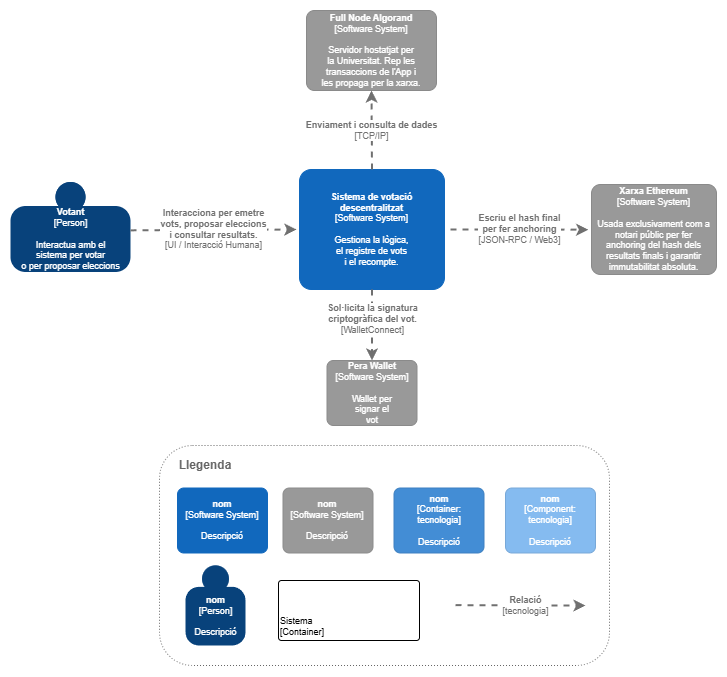
\includegraphics[width=0.85\textwidth]{images/c4-n1.png} 
    \caption{Diagrama de context del sistema (Nivell 1 del model C4).}
    \label{fig:c4-nivell-1}
\end{figure}
 
\subsection{Contenidors del sistema (Nivell 2)}
 
El sistema es descompon en cinc contenidors principals, cadascun amb una responsabilitat ben delimitada i un acoblament mínim amb la resta:
 
\subsubsection{Aplicació web \textit{(\textit{front-end}})}
 
Aplicació d'una sola pàgina (\textit{Single-Page Application}) que el votant descarrega des d'un repositori oficial i executa localment. Desenvolupada amb React i empaquetada amb Vite, és responsable de renderitzar la interfície d'usuari, mostrar les eleccions actives, empaquetar el vot en format de transacció Algorand (ApplicationCall) i enviar-lo al node. L'aplicació no emmagatzema cap dada sensible i opera com un client lleuger (\textit{thin client}) que delega tota la lògica de negoci al contracte intel·ligent.
 
El flux d'interacció de l'usuari segueix una seqüència de quatre passos: (1) l'usuari ordena els candidats per preferència mitjançant \textit{drag and drop}, (2) l'aplicació empaqueta l'ordre de preferències en format de transacció Algorand, (3) sol·licita la signatura criptogràfica a la cartera digital i (4) envia la transacció signada al node complet d'Algorand perquè la propagui a la xarxa.

 
\subsubsection{Node Complet d'Algorand}
 
Servidor hostatjat per la universitat (o, en un escenari productiu, per les entitats institucionals participants) que rep les transaccions de l'aplicació web i les propaga per la xarxa blockchain. Implementat en Go, exposa una API REST estàndard compatible amb l'Algorand SDK. La seva funció és exclusivament la de punt d'entrada a la xarxa: no conté lògica de negoci pròpia ni té accés a les claus dels votants.
 
 
\subsubsection{Smart Contract de Votació}
 
Lògica immutable desplegada a la xarxa Algorand, escrita en PyTeal i compilada a TEAL (Transaction Execution Approval Language). Constitueix el nucli del sistema i la peça que elimina la necessitat de confiança en cap autoritat central. Les seves responsabilitats són:
 
\begin{enumerate}[label=\roman*.]
    \item Votacions d'eleccions.
    \item Generació i emmagatzematge de propostes d'eleccions.
    \item Validació del cens electoral i verificació de permisos (verificació que l'adreça del votant pertany a la llista blanca i que l'acció sol·licitada pot ser realitzada).
    \item Prevenció del doble vot.
    \item Gestió del cicle de vida de l'elecció (dates d'inici i finalització).
    \item Recompte automàtic i transparent dels vots.
\end{enumerate}
 
L'estat del contracte s'emmagatzema emprant dos mecanismes natius d'Algorand: \textbf{Box Storage} per guardar les propostes i el recompte global de vots, i \textbf{Global State} per registrar si un votant concret ja ha exercit el seu dret, evitant així el doble vot sense revelar l'opció seleccionada.
 
\subsubsection{Servei d'Anchoring}
 
Component automatitzat que cada entitat que opera un node complet (\textit{full node}) ha d'executar. Aquest servei llegeix l'estat de les votacions des del node d'Algorand via l'AlgoSDK REST API i, quan una elecció finalitza, genera el \textit{hash} SHA-256 de l'estat de la blockchain corresponent a l'escrutini. Seguidament, envia aquest \textit{hash} signat a un contracte intel·ligent propi desplegat a la xarxa pública d'Ethereum (Sepolia Testnet) mitjançant JSON-RPC.

El contracte d'Ethereum (escrit en Solidity) actua com una ``cort suprema'' descentralitzada: manté una llista blanca d'adreces de wallet universitàries autoritzades i implementa una lògica de consens amb llindar (\textit{\textit{K-of-N}}). Només quan K universitats independents acorden un \textit{hash} d'estat idèntic, el contracte ancora el resultat final de l'elecció al registre d'Ethereum, evitant així el frau per punt únic de fallada.

\subsubsection{Pera Wallet (sistema extern)}
 
Cartera digital mòbil de l'ecosistema Algorand que actua com a custòdia exclusiva de les claus privades del votant. El sistema interactua amb Pera Wallet a través del protocol WalletConnect: l'aplicació web genera un codi QR, l'usuari l'escaneja, i la cartera retorna la transacció signada criptogràficament sense que la clau privada abandoni mai el dispositiu mòbil de l'elector.

\begin{figure}[H]
    \centering
    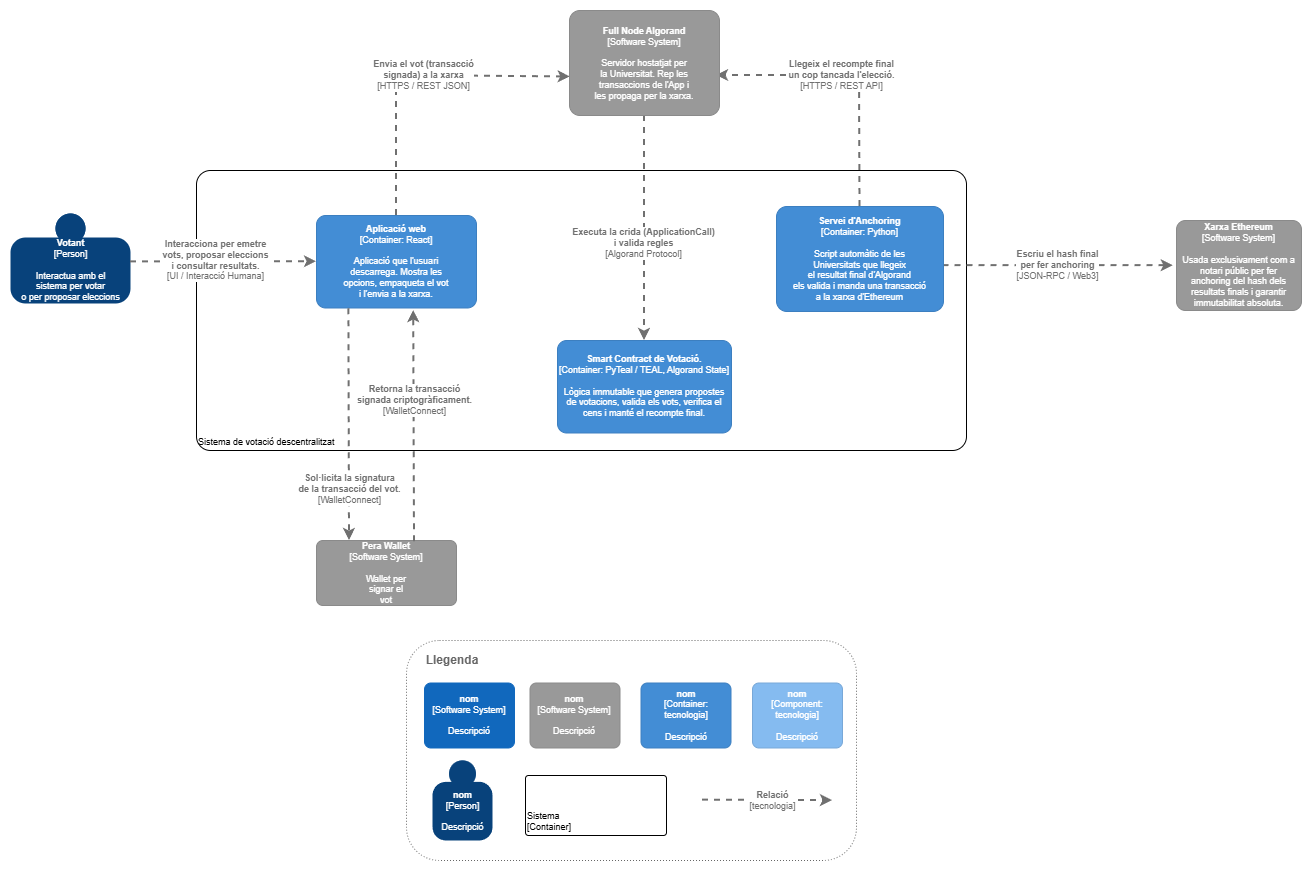
\includegraphics[width=0.85\textwidth]{images/c4-n2.png} 
    \caption{Diagrama de contenidors del sistema (Nivell 2 del model C4).}
    \label{fig:c4-nivell-2}
\end{figure}

\subsection{Components interns (Nivell 3)}
 
A continuació es detalla la descomposició interna dels tres contenidors desenvolupats per l'equip del projecte: l'aplicació web, el contracte intel·ligent i el servei d'anchoring.
 
\subsubsection{Components de l'aplicació web}

L'aplicació React es descompon en quatre capes principals amb responsabilitats clarament separades:

\begin{enumerate}[label=\roman*.]
    \item \textbf{Capa de presentació} (\textit{React Components}): conté set vistes (\texttt{Landing}, \texttt{Dashboard}, \texttt{Elections}, \texttt{Proposals}, \texttt{Voting}, \texttt{Results} i \texttt{Verification}), cadascuna amb els seus propis fitxers JSX i CSS. Els components reutilitzables d'interfície (\texttt{Button}, \texttt{Card}, \texttt{DraggableList}, \texttt{Timeline}, \texttt{DotGrid}) i els de disposició (\texttt{Navbar}, \texttt{PageWrapper}) s'agrupen per separat. El disseny segueix una estètica \textit{glassmorphism} amb mode clar i fosc.

    \item \textbf{Capa d'internacionalització} (\textit{react-i18next}): tota la interfície està disponible en anglès, espanyol i català mitjançant fitxers de traducció JSON. El sistema detecta automàticament l'idioma del navegador i permet canviar-lo manualment des de la barra de navegació.

    \item \textbf{Mòdul WalletConnect} (\textit{WalletConnect SDK}): gestiona la sessió amb Pera Wallet, genera el codi QR per establir la connexió i envia les sol·licituds de signatura a l'usuari. Encapsula tota la complexitat del protocol de comunicació amb la cartera.

    \item \textbf{Generador de transaccions} (\textit{Algorand JS SDK --- algosdk}): tradueix les accions de l'usuari (``Votar opció A'' o ``Proposar elecció X'') en transaccions \textit{byte-code} d'Algorand (ApplicationCall) a punt per ser signades. Aquesta capa d'abstracció garanteix que la resta de l'aplicació no necessita conèixer els detalls de baix nivell del protocol Algorand.
\end{enumerate}

El flux de navegació de l'aplicació comença amb una pàgina d'aterratge (\texttt{Landing}), des de la qual l'usuari accedeix al tauler de control (\texttt{Dashboard}). Des d'allà pot consultar eleccions actives i passades (\texttt{Elections}), redactar propostes (\texttt{Proposals}), emetre el seu vot mitjançant un sistema D\&D amb mètode Schulze (\texttt{Voting}), consultar resultats amb la matriu de comparació per parells (\texttt{Results}) i verificar el seu vot a la cadena de blocs (\texttt{Verification}).

La capa de presentació sol·licita accions al generador de transaccions, que construeix la transacció i demana la signatura al mòdul WalletConnect. Un cop la cartera retorna la transacció signada, el generador l'envia directament al node complet d'Algorand mitjançant HTTPS/REST JSON.

\begin{figure}[H]
    \centering
    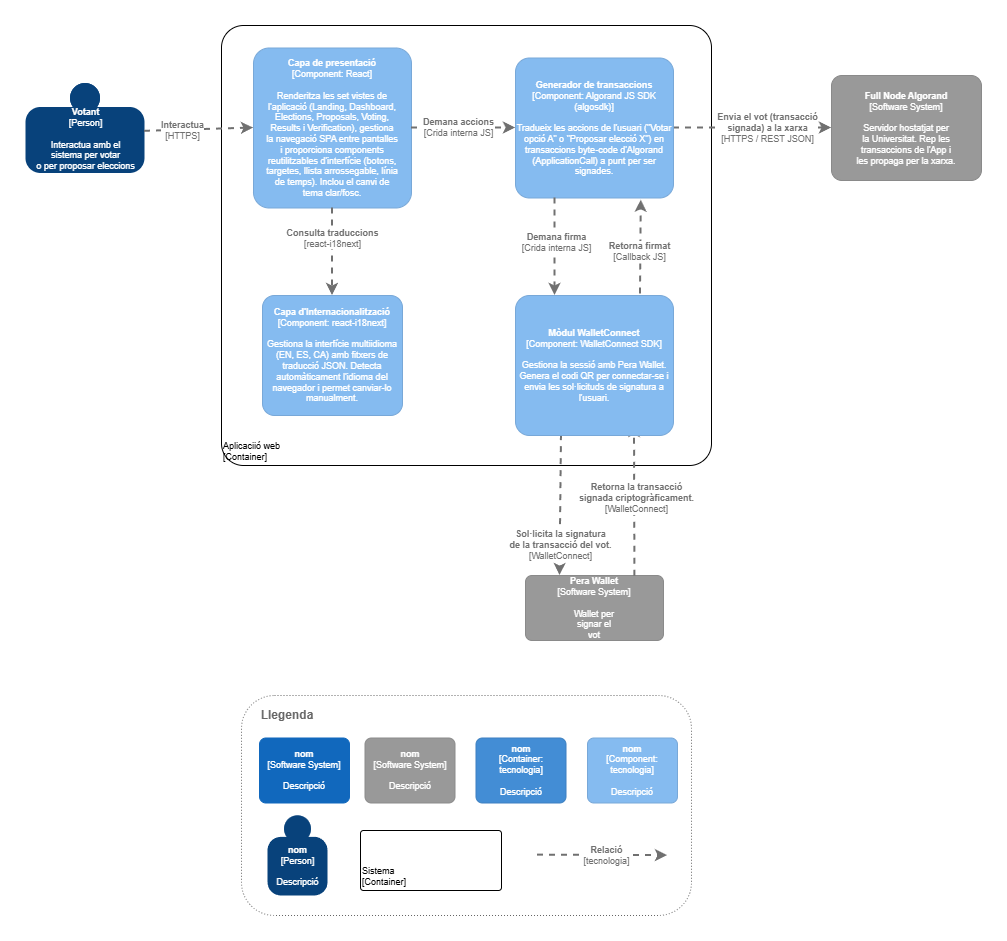
\includegraphics[width=0.85\textwidth]{images/c4-n3-app.png} 
    \caption{Components de l'aplicació web (Nivell 3 del model C4).}
    \label{fig:c4-nivell-3-app}
\end{figure}


\subsubsection{Components del Smart Contract}
 
El contracte intel·ligent es descompon internament en sis mòduls lògics. La interacció entre el node Algorand i el contracte segueix l'estàndard ABI d'Algorand (ARC-4), que defineix la codificació dels arguments i els valors de retorn de cada crida:
 
\begin{enumerate}[label=\roman*.]
    \item \textbf{Enrutador principal} (\textit{PyTeal Cond}): punt d'entrada del contracte. Rep cada transacció i, segons els arguments de l'ApplicationCall, la redirigeix al mòdul de votació, al de propostes o al generador d'eleccions. Implementa el patró \textit{Router} per centralitzar el control del flux d'execució.

    \item \textbf{Verificador} (\textit{PyTeal}): encarregat de verificar que l'acció sol·licitada a la transacció pugui ser realitzada. Comprova que l'acció no s'hagi realitzat amb anterioritat (per exemple, que l'usuari no hagi votat ja) i revisa que la \textit{wallet} que ha signat la transacció tingui permisos per executar l'operació sol·licitada (pertinença al cens). La comunicació amb l'emmagatzematge d'estat es fa mitjançant les operacions \texttt{box\_get()} del protocol Box Opcode d'Algorand. L'enrutador delega la validació a aquest mòdul mitjançant crides internes (\texttt{CallSub}).

    \item \textbf{Lògica de propostes} (\textit{PyTeal}): encarregat de comunicar-se amb l'estat del contracte per registrar una proposta d'elecció. Defineix les dates d'inici i finalització, el nom de la proposta, els participants i les entitats o opcions a ser elegides. L'escriptura a l'estat es realitza mitjançant actualitzacions atòmiques (\texttt{app\_global\_put()}).

    \item \textbf{Lògica de votació} (\textit{PyTeal}): encarregat de comunicar-se amb l'estat del contracte per modificar el recompte de vots. L'escriptura d'increments de vot es fa mitjançant actualitzacions atòmiques (\texttt{app\_global\_put()}) que garanteixen la consistència de l'estat.

    \item \textbf{Generador d'eleccions} (\textit{PyTeal}): llegeix l'estat del contracte (els vots de les propostes d'eleccions mitjançant \texttt{box\_get()}) i, si una proposta ha assolit un llindar determinat de vots favorables, genera automàticament les eleccions corresponents mitjançant transaccions internes (\texttt{itxn.submit()}). Implementa la lògica de transició entre la fase de proposta i la fase electoral. La lògica de propostes notifica aquest mòdul mitjançant \texttt{CallSub()} cada cop que es registra un nou vot a una proposta.

    \item \textbf{Emmagatzematge d'estat} (\textit{Algorand Box Storage \& Local State}): base de dades del contracte. Guarda les propostes (Box Storage), el recompte de vots per proposta, el recompte de vots per elecció (Global/Box) i el registre individual de qui ha votat (Local State per evitar el doble vot).
\end{enumerate}

\begin{figure}[H]
    \centering
    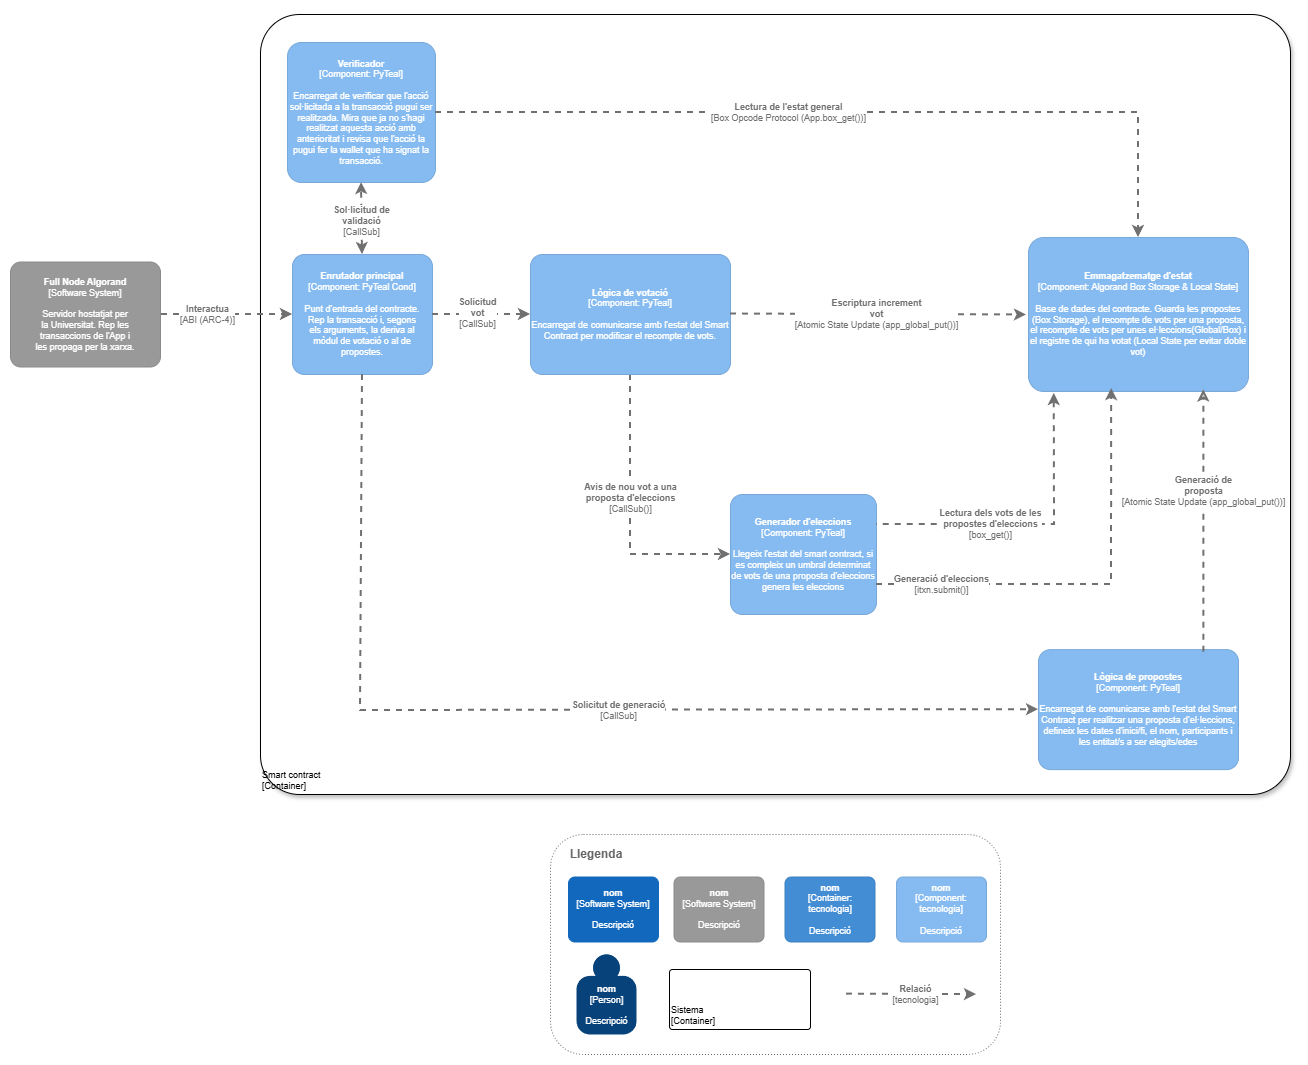
\includegraphics[width=0.85\textwidth]{images/c4-n3-smart-contract.png} 
    \caption{Components del Smart Contract (Nivell 3 del model C4).}
    \label{fig:c4-nivell-3-sc}
\end{figure}

\subsubsection{Components del Servei d'Anchoring}

El servei d'anchoring es descompon en dos components que operen conjuntament per materialitzar l'ancoratge distribuït dels resultats:

\begin{enumerate}[label=\roman*.]
    \item \textbf{Gestor d'ancoratge} (\textit{Python}): mòdul encarregat de revisar l'estat de les votacions consultant el node d'Algorand via l'AlgoSDK REST API. Quan una votació finalitza, aquest component genera el \textit{hash} SHA-256 de l'estat de la blockchain corresponent a l'escrutini i l'envia, signat criptogràficament (ECDSA), al contracte d'Ethereum mitjançant JSON-RPC.

    \item \textbf{Ethereum Notary Contract} (\textit{Solidity}): contracte intel·ligent desplegat a la xarxa Ethereum (Sepolia Testnet), dissenyat i implementat pel propi equip del projecte. Actua com una ``cort suprema'' descentralitzada que manté una \textit{whitelist} d'adreces de wallet universitàries autoritzades i implementa una lògica de consens amb llindar (\textit{\textit{K-of-N}}). Agrega els \textit{hash}es d'estat provinents dels nodes universitaris i només ancora el resultat final de l'elecció al registre d'Ethereum quan K universitats independents acorden un \textit{hash} d'estat idèntic, evitant així el frau per punt únic de fallada. Les funcionalitats del contracte inclouen: mantenir la llista d'adreces autoritzades (afegir i eliminar), rebre transaccions dels nodes autoritzats i, si se supera el llindar de coincidència, publicar el \textit{hash} a la xarxa.
\end{enumerate}

\begin{figure}[H]
    \centering
    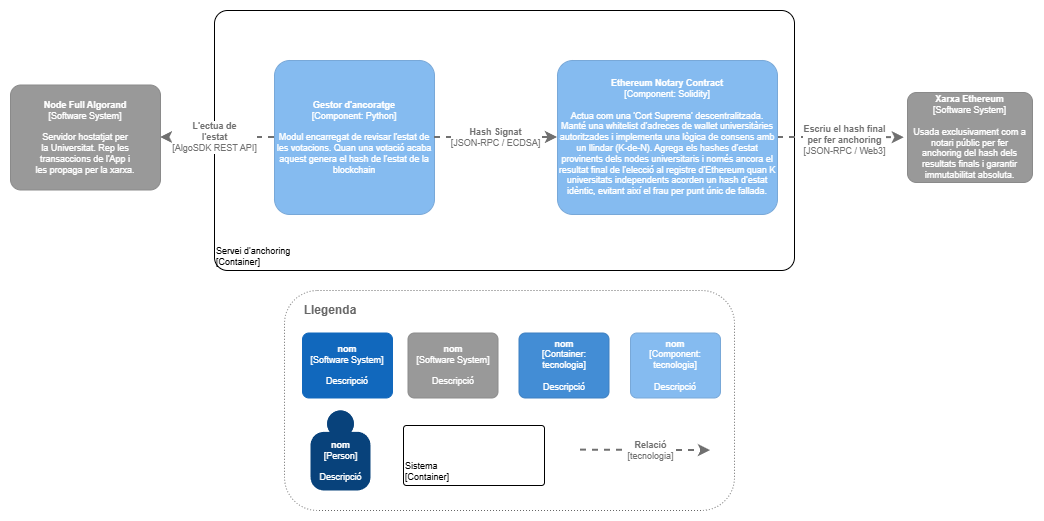
\includegraphics[width=0.85\textwidth]{images/c4-n3-servei-anchoring.png} 
    \caption{Components del Servei d'Anchoring (Nivell 3 del model C4).}
    \label{fig:c4-nivell-3-anchoring}
\end{figure}


% ===========================================================================
%   SECCIÓ 9 - TECNOLOGIES I SOFTWARE DE TERCERS
% ===========================================================================
\section{Tecnologies i software de tercers}
 
El sistema s'ha construït emprant exclusivament eines de codi obert i plataformes gratuïtes, en coherència amb el requisit de projecte d'incórrer en zero despesa econòmica (secció 3.3.3 del document d'abast). Cada tecnologia s'ha seleccionat atenent a criteris de maduresa, documentació disponible, compatibilitat amb l'ecosistema Algorand i accessibilitat per a l'equip de desenvolupament. A continuació es descriuen les tecnologies emprades, agrupades per capa del sistema.
 
\subsection{Capa de blockchain i contractes intel·ligents}
 
\subsubsection{Algorand (protocol de consens)}
 
Algorand és la xarxa blockchain seleccionada com a infraestructura del sistema de votació. Utilitza un mecanisme de consens basat en Pure Proof of Stake (PPoS) combinat amb una Funció Aleatòria Verificable (VRF) que garanteix que la selecció de validadors és aleatòria, impredictible i verificable criptogràficament. Les seves propietats fonamentals per al projecte són: finalitat immediata de les transaccions (sense possibilitat de \textit{forks}), comissions de transacció negligibles (0,001 ALGO), i suport natiu per a contractes intel·ligents amb emmagatzematge d'estat (Global State, Local State i Box Storage).
 
La decisió d'emprar Algorand en lloc d'Ethereum per a la lògica de votació es justifica per tres raons: (1) la finalitat instantània elimina la incertesa sobre si un vot ha estat confirmat, (2) el cost per transacció és ordres de magnitud inferior al gas d'Ethereum, fent viable un sistema on cada vot és una transacció, i (3) el model d'emmagatzematge natiu (Box Storage) permet estructures de dades complexes directament al contracte sense necessitat de mapejar tot a \textit{storage slots} de 256 bits.
 
\subsubsection{PyTeal / TEAL}
 
PyTeal és una llibreria de Python que permet escriure contractes intel·ligents per a Algorand emprant sintaxi Python nativa, que posteriorment es compila a TEAL (\textit{Transaction Execution Approval Language}), el llenguatge d'assembler de la màquina virtual d'Algorand (AVM). L'elecció de PyTeal per sobre d'alternatives com Puya (Algorand Python) es basa en la major maduresa de la seva documentació i la disponibilitat d'exemples dins la comunitat, factors crítics donada la corba d'aprenentatge prevista a la gestió de riscos (secció 6.4).
 
Tot el codi dels contractes (lògica de propostes, votació, verificació, generació d'eleccions i enrutament) s'escriu en PyTeal i es compila a TEAL abans del desplegament. La interacció amb el contracte segueix l'estàndard ABI d'Algorand (ARC-4), que defineix la codificació dels arguments de cada crida. Aquesta separació entre el llenguatge de desenvolupament (Python) i el d'execució (TEAL) facilita les proves unitàries i la lectura del codi per part d'auditors.
 
\subsubsection{AlgorKit (AlgoKit)}
 
AlgorKit és l'eina oficial de la Fundació Algorand per a la gestió del cicle de vida complet dels projectes blockchain: creació de l'entorn local, desplegament de contractes, execució de proves i interacció amb la xarxa. En el context d'aquest projecte, s'empra per aixecar una xarxa Algorand local simulada dins un contenidor Docker amb una única comanda, permetent iterar ràpidament sobre el codi dels contractes sense incórrer en costos de xarxa.
 
AlgorKit proporciona comptes prefabricats amb saldos de prova, un indexer local per a consultes, i una CLI que automatitza les tasques repetitives de desplegament. Constitueix la peça clau per complir el requisit de reproducibilitat (secció 3.2.1): qualsevol membre de l'equip pot replicar l'entorn exacte clonant el repositori i executant \texttt{algokit localnet start}.

\subsubsection{Solidity (contracte d'Ethereum)}

Solidity és el llenguatge de programació emprat per escriure el contracte intel·ligent d'ancoratge desplegat a la xarxa Ethereum (Sepolia Testnet). Aquest contracte, denominat \textit{Ethereum Notary Contract}, implementa la lògica de consens amb llindar \textit{K-of-N} que agrega els \textit{hash}es enviats pels nodes universitaris. S'ha seleccionat Solidity per ser el llenguatge estàndard i més madur de l'ecosistema Ethereum, amb àmplia documentació i suport d'eines de desenvolupament com Hardhat o Remix.
 
\subsection{Capa de \textit{front-end}}
 
\subsubsection{React}
 
React (versió 19) és la llibreria de JavaScript seleccionada per al desenvolupament de la interfície d'usuari. La seva arquitectura basada en components reactius i el seu model de flux de dades unidireccional permeten mantenir una separació neta entre la presentació visual i la lògica d'estat de l'aplicació. L'equip compta amb experiència prèvia en React, la qual cosa redueix la corba d'aprenentatge i permet concentrar l'esforç en la integració \textit{blockchain}.
 
\subsubsection{Vite}
Vite és l'eina de construcció (\textit{build tool}) i servidor de desenvolupament emprada per al \textit{front-end}. Substitueix la configuració tradicional basada en Webpack i Create React App, oferint arrancades quasi instantànies gràcies al seu mode de servei basat en mòduls ES natius i una compilació de producció optimitzada mitjançant Rollup. El contenidor Docker del \textit{front-end} utilitza Bun com a \textit{runtime} alternatiu a Node.js per accelerar la instal·lació de dependències i l'execució del servidor de desenvolupament.

\subsubsection{react-i18next}
El sistema d'internacionalització es basa en la llibreria \texttt{react-i18next} combinada amb \texttt{i18next-browser-languagedetector}. Tota la interfície està disponible en tres idiomes (anglès, espanyol i català) mitjançant fitxers de traducció JSON separats per \textit{locale}. El detector d'idioma identifica automàticament la preferència del navegador de l'usuari i permet el canvi manual d'idioma des de la barra de navegació.
 
\subsubsection{Algorand JavaScript SDK (algosdk)}
 
La llibreria oficial \texttt{algosdk} permet a l'aplicació web construir, signar i enviar transaccions d'Algorand des del navegador. S'empra per traduir les accions de l'usuari en transaccions \textit{ApplicationCall} byte-code compatibles amb el contracte intel·ligent, seguint l'estàndard ABI (ARC-4). La versió emprada suporta la construcció de transaccions atòmiques (grups de transaccions) i la interacció amb Box Storage.
 
\subsubsection{WalletConnect SDK}
 
WalletConnect és el protocol de comunicació estàndard entre aplicacions web (dApps) i carteres digitals mòbils. El SDK s'integra a l'aplicació React per generar codis QR de connexió, establir sessions xifrades amb Pera Wallet i enviar sol·licituds de signatura. Totes les comunicacions entre l'aplicació i la cartera es xifren mitjançant un pont (\textit{bridge}) independent, garantint que la clau privada del votant mai transita per la xarxa de l'aplicació.
 
\subsection{Capa d'anchoring i auditoria}
 
\subsubsection{Ethereum (Sepolia Testnet)}
 
La xarxa pública d'Ethereum s'empra exclusivament com a notari públic extern. El servei d'anchoring de cada node institucional envia el \textit{hash} SHA-256 dels resultats finals al contracte d'Ethereum Notary desplegat a la Sepolia Testnet, que aplica la lògica de consens amb llindar abans de publicar el resultat. La selecció de Sepolia en lloc d'altres testnets (Goerli, ja obsoleta) segueix la recomanació oficial de la Fundació Ethereum per a aplicacions de prova.
 
\subsubsection{Web3.py}
 
Llibreria de Python que proporciona la interfície de comunicació amb la xarxa Ethereum mitjançant el protocol JSON-RPC. S'empra dins el gestor d'ancoratge per construir i enviar la transacció que conté el \textit{hash} de l'escrutini al contracte Notary. La seva compatibilitat nativa amb Sepolia i la seva àmplia documentació la fan la solució més directa per a l'escriptura de dades a Ethereum des d'un script Python.
 
\subsection{Capa d'infraestructura i desplegament}
 
\subsubsection{Docker}
 
Docker és l'eina central de contenidorització del projecte. Permet empaquetar tots els serveis del sistema (node Algorand, servidor \textit{front-end}, servei d'anchoring) en contenidors independents i reproduïbles. Cada component es defineix en un \texttt{Dockerfile} propi i l'orquestració del conjunt es gestiona amb \texttt{docker-compose}, garantint que qualsevol desenvolupador o avaluador pugui desplegar el sistema complet amb una única comanda.
 
\subsubsection{Git i GitHub}
 
El sistema de control de versions es gestiona amb Git, i el repositori central s'allotja a GitHub. L'estratègia de branques segueix el model Trunk Based Development descrit a la secció 7.2 del document d'abast, amb branques de funcionalitat curtes que s'integren a \texttt{main} mitjançant Pull Requests revisades.
 
\subsection{Resum de tecnologies}
 
La taula~\ref{tab:tecnologies} resumeix totes les tecnologies emprades, la seva capa dins l'arquitectura i la seva funció específica.
 
\begin{table}[H]
\centering
\small
\begin{tabularx}{\textwidth}{l l X}
\toprule
\textbf{Tecnologia} & \textbf{Capa} & \textbf{Funció dins el sistema} \\
\midrule
Algorand (PPoS/VRF) & Blockchain & Xarxa on resideix el contracte de votació \\
PyTeal / TEAL & Blockchain & Escriptura i compilació dels contractes intel·ligents d'Algorand \\
ARC-4 (ABI) & Blockchain & Estàndard d'interfície per a les crides al contracte \\
AlgorKit & Blockchain & Entorn local simulat i CLI de desplegament \\
Solidity & Blockchain & Escriptura del contracte d'anchoring a Ethereum \\
React & \textit{front-end} & Interfície d'usuari de l'aplicació de votació \\
Vite 8 & \textit{front-end} & Eina de construcció i servidor de desenvolupament \\
react-i18next & \textit{front-end} & Internacionalització en anglès, espanyol i català \\
algosdk (JS) & \textit{front-end} & Construcció de transaccions Algorand des del navegador \\
WalletConnect SDK & \textit{front-end} & Protocol de comunicació segura amb Pera Wallet \\
Pera Wallet & Externa & Custòdia de claus privades i signatura de transaccions \\
Ethereum (Sepolia) & Anchoring & Notari públic per a l'ancoratge del \textit{hash} dels resultats \\
Web3.py & Anchoring & Interfície Python per a la interacció amb Ethereum \\
Docker & Infraestructura & Contenidorització i reproducibilitat de l'entorn \\
Git / GitHub & Infraestructura & Control de versions i col·laboració \\
\bottomrule
\end{tabularx}
\caption{Resum de tecnologies i software de tercers emprats al projecte}
\label{tab:tecnologies}
\end{table}
 
 
% ===========================================================================
%   SECCIÓ 10 - DECISIONS TÈCNIQUES (PATRONS DE DISSENY)
% ===========================================================================
\section{Decisions tècniques (patrons de disseny)}
 
Les decisions tècniques del projecte no responen a criteris arbitraris, sinó a la necessitat de resoldre problemes concrets derivats dels requisits funcionals i no funcionals establerts a la secció 3 del document d'abast. Cada decisió es presenta juntament amb el problema que resol, les alternatives considerades i la justificació de l'opció triada.
 
\subsection{Patró Router per al contracte intel·ligent}
 
\textbf{Problema}: un contracte intel·ligent d'Algorand rep totes les transaccions a través d'un únic punt d'entrada (l'Approval Program). Cal un mecanisme per distingir si una transacció és un vot, una proposta, una consulta de resultats o una sol·licitud de generació d'eleccions.
 
\textbf{Solució}: s'implementa un enrutador principal (patró \textit{Router}) al començament del codi PyTeal que inspecciona els arguments de l'ApplicationCall (\texttt{Txn.application\_args[0]}) i, mitjançant una estructura condicional (\texttt{Cond}), redirigeix l'execució al mòdul corresponent: verificador, lògica de votació, lògica de propostes o generador d'eleccions.
 
\textbf{Justificació}: aquest patró centralitza el control de flux, facilita l'extensibilitat del contracte (afegir noves funcionalitats sense modificar els mòduls existents) i millora la llegibilitat del codi, ja que cada mòdul gestiona una única responsabilitat. A més, segueix el principi de responsabilitat única (\textit{Single Responsibility Principle}) dins les restriccions de la AVM, que no permet herència ni modularització a nivell de fitxers.

\subsection{Verificació desacoblada de la lògica de negoci}

\textbf{Problema}: cada operació del contracte (votar, proposar, generar eleccions) requereix verificar que l'usuari té permisos (pertany al cens) i que l'acció no s'ha realitzat amb anterioritat (prevenció del doble vot o doble proposta). Si aquesta lògica es duplica dins de cada mòdul, qualsevol error o inconsistència en una de les còpies crea una vulnerabilitat.

\textbf{Solució}: s'implementa un mòdul \textbf{Verificador} independent que centralitza totes les comprovacions de permisos i duplicació. L'enrutador delega la validació a aquest mòdul mitjançant crides internes (\texttt{CallSub}) abans de transferir el control al mòdul funcional corresponent. El verificador consulta l'estat general del contracte mitjançant les operacions del protocol Box Opcode (\texttt{box\_get()}).

\textbf{Justificació}: el desacoblament de la verificació respecte de la lògica de negoci proporciona un únic punt d'auditoria per a totes les regles de control d'accés. Si cal modificar la política de verificació (per exemple, canviar el criteri de pertinença al cens), només cal actualitzar un mòdul en lloc de revisar tots els fluxos del contracte. Aquesta separació segueix el patró \textit{Guard} o \textit{Middleware}, adaptat a les restriccions de la AVM.
 
\subsection{Separació d'estat: Box Storage vs. Local State}
 
\textbf{Problema}: el contracte necessita emmagatzemar dos tipus de dades amb requisits d'accés molt diferents: (1) informació global compartida (propostes d'elecció, recomptes de vots, dates) i (2) informació individual per votant (si ha votat o no en una elecció concreta).
 
\textbf{Solució}: les dades globals s'emmagatzemen en \textbf{Box Storage}, que ofereix espai d'emmagatzematge de mida variable associat al contracte, adequat per a estructures de dades complexes com llistes de propostes o mapeigs de recompte. Les dades individuals de cada votant es registren al \textbf{Local State}, que és un espai d'emmagatzematge lligat al compte de l'usuari que ha fet \textit{opt-in} al contracte, perfecte per registrar un \textit{flag} booleà de ``ha votat''.
 
\textbf{Justificació}: aquesta separació explota les propietats natives d'Algorand de manera òptima. El Local State permet verificar el doble vot amb una sola lectura (O(1)) sense necessitat d'iterar una llista de votants al Box Storage, cosa que seria inviable dins els límits d'opcode de la AVM. A més, el Local State és privat del compte de l'usuari, proporcionant una capa addicional de separació entre la identitat del votant i la seva acció.

\subsection{Operacions atòmiques per a la consistència de l'estat}

\textbf{Problema}: les operacions d'escriptura al contracte (registre d'un vot, creació d'una proposta, generació d'una elecció) modifiquen múltiples camps de l'estat. Si una operació falla a mig camí, l'estat del contracte podria quedar en un estat inconsistent.

\textbf{Solució}: totes les escriptures a l'estat del contracte es realitzen mitjançant actualitzacions atòmiques (\texttt{app\_global\_put()}) que garanteixen que l'operació es completa íntegrament o no es realitza en absolut. Per a la generació d'eleccions a partir de propostes, s'empren transaccions internes (\texttt{itxn.submit()}) que permeten al contracte crear noves estructures de dades dins la mateixa transacció.

\textbf{Justificació}: l'atomicitat és un requisit fonamental en sistemes on cada operació (vot) té implicacions legals i de confiança. Un recompte inconsistent invalidaria tot el procés electoral. L'ús de les primitives atòmiques natives d'Algorand elimina aquesta classe d'errors per disseny.
 
\subsection{Thin Client: delegació completa de lògica al contracte}
 
\textbf{Problema}: si l'aplicació web conté lògica de validació duplicada (per exemple, comprovar el cens o verificar dates), existeix un risc de discrepància entre el comportament del \textit{front-end} i el del contracte, a més de crear un vector d'atac si un usuari maliciós modifica el codi client.
 
\textbf{Solució}: l'aplicació web opera com un \textit{Thin Client} que no implementa cap regla de negoci. Tota la validació (cens, doble vot, finestra temporal, increment de comptadors) resideix exclusivament al contracte intel·ligent. El \textit{front-end} es limita a construir transaccions, sol·licitar signatures i mostrar resultats.
 
\textbf{Justificació}: en un sistema on la confiança es resol per disseny, el codi executable de referència ha de ser únic i residir a la blockchain. Si la validació del cens estigués al \textit{front-end}, un atacant podria modificar el JavaScript i intentar emetre transaccions invàlides. Amb el model \textit{Thin Client}, qualsevol transacció que no compleixi les regles del contracte serà rebutjada per la xarxa independentment del que faci l'aplicació client.
 
\subsection{Signatura delegada i principi de mínim privilegi}
 
\textbf{Problema}: el sistema necessita que les transaccions estiguin signades criptogràficament amb la clau privada del votant, però cap component de la infraestructura pot tenir accés a aquesta clau.
 
\textbf{Solució}: s'aplica el principi de mínim privilegi delegant completament la signatura a Pera Wallet mitjançant WalletConnect. L'aplicació web construeix la transacció (no signada), l'envia a la cartera, i rep de tornada la transacció signada per propagar-la al node. En cap moment la clau privada abandona el dispositiu mòbil del votant.
 
\textbf{Justificació}: la gestió incorrecta de claus privades és el vector d'atac més comú en aplicacions descentralitzades. Delegar la signatura a una cartera especialitzada elimina de soca-rel la possibilitat que un servidor compromès o un error al \textit{front-end} exposi les credencials del votant. A més, aquest model és transparent per a l'usuari: l'acció de signar un vot es percep com una confirmació al mòbil, similar a la validació biomètrica d'una aplicació bancària.
 
\subsection{Ancoratge distribuït amb consens \textit{K-of-N} (Cross-chain Anchoring)}
 
\textbf{Problema}: en el plantejament inicial, un únic servei centralitzat era l'encarregat de llegir l'estat d'Algorand i escriure'l a Ethereum. Això introduïa un punt únic de fallada: si el servei estava compromès o produïa un \textit{hash} incorrecte, l'ancoratge no oferia cap garantia real. Cal un mecanisme que proporcioni un segell de temps independent, verificable i resistent a la manipulació per part d'una única entitat.
 
\textbf{Solució}: cada entitat que opera un node complet calcula independentment el \textit{hash} SHA-256 de l'estat final de l'escrutini i l'envia a un contracte intel·ligent desplegat a Ethereum (Sepolia Testnet). Aquest contracte, escrit en Solidity i dissenyat pel propi equip, implementa una lògica de consens amb llindar: manté una llista blanca d'adreces autoritzades (les wallet universitàries) i només ancora el \textit{hash} com a resultat oficial quan K de N nodes independents han enviat el mateix valor.
 
\textbf{Justificació}: el model \textit{K-of-N} elimina el punt únic de fallada de l'ancoratge i alinea el servei amb el principi de descentralització que fonamenta tot el sistema. Ethereum, com a xarxa pública amb milers de nodes independents, actua com a notari públic extern. Si un atacant comprometés un node universitari i enviés un \textit{hash} fals, aquest no coincidiria amb els \textit{hash}es de la resta de nodes i el contracte d'Ethereum no l'ancoraria. Per manipular l'ancoratge caldria comprometre K nodes simultàniament, cosa criptogràficament inviable en la pràctica.
 
\subsection{Resum de decisions tècniques}
 
La taula~\ref{tab:decisions} sintetitza les decisions de disseny principals i la seva traçabilitat amb els requisits del sistema.
 
\begin{table}[H]
\centering
\small
\begin{tabularx}{\textwidth}{l l X}
\toprule
\textbf{Decisió} & \textbf{Patró} & \textbf{Requisit que resol} \\
\midrule
Enrutador del contracte & Router & RF 3.1.2, 3.1.3 \\
Verificació desacoblada & Guard / Middleware & RF 3.1.1 (cens), RF 3.1.2 (doble vot) \\
Separació Box/Local State & Strategy (Storage) & RF 3.1.2 (doble vot), RF 3.1.4 \\
Operacions atòmiques & Atomic Transaction & RF 3.1.4 (integritat recompte) \\
Thin Client & Client-Server & RNF 3.2.5 (seguretat) \\
Signatura delegada & Mínim privilegi & RNF 3.2.5 (credencials) \\
Ancoratge \textit{K-of-N} & Cross-chain Consensus & RF 3.1.5 (immutabilitat) \\
\bottomrule
\end{tabularx}
\caption{Traçabilitat entre decisions tècniques i requisits del sistema}
\label{tab:decisions}
\end{table}
 
 
% ===========================================================================
%   SECCIÓ 11 - ESTRATÈGIA DE DESPLEGAMENT
% ===========================================================================
\section{Estratègia de desplegament}
 
L'estratègia de desplegament defineix com el sistema es construeix, es posa en marxa i es valida en cada una de les seves fases. Donada la naturalesa acadèmica del projecte i la restricció de zero cost econòmic, tot el desplegament es basa en entorns locals simulats i xarxes de prova públiques gratuïtes.
 
\subsection{Entorn de desplegament local}
 
L'entorn de desenvolupament i proves es basa en una xarxa Algorand local simulada, gestionada íntegrament per AlgorKit i orquestrada amb Docker. L'objectiu és que qualsevol desenvolupador o avaluador pugui reproduir el sistema complet amb un esforç mínim de configuració.
 
El procés de posada en marxa segueix una seqüència determinista:
 
\begin{enumerate}[label=\roman*.]
    \item \textbf{Inicialització de la xarxa}: s'executa \texttt{algokit localnet start}, que aixeca un parell de nodes Algorand complet, un indexer i un KMD (\textit{Key Management Daemon}) dins contenidors Docker. Aquesta comanda crea automàticament comptes de prova amb saldos suficients per a les transaccions.
    \item \textbf{Desplegament del contracte d'Algorand}: es compila el codi PyTeal a TEAL i es desplega el contracte intel·ligent de votació a la xarxa local mitjançant la CLI d'AlgorKit (\texttt{algokit deploy}). El procés retorna l'identificador (App ID) del contracte desplegat.
    \item \textbf{Desplegament del contracte d'Ethereum}: es desplega l'Ethereum Notary Contract a la Sepolia Testnet (o a una xarxa Ethereum local per a proves), configurant la llista d'adreces autoritzades i el llindar \textit{K-of-N}.
    \item \textbf{Configuració del cens}: un script de Python pobla el contracte amb una llista blanca d'adreces de prova que simulen el cens electoral autoritzat.
    \item \textbf{Arrancada del \textit{front-end}}: l'aplicació React s'inicia amb \texttt{npm run dev} (o dins un contenidor Docker propi basat en Bun: \texttt{docker-compose up \textit{front-end}}) i es configura perquè apunti al node local d'Algorand i a l'App ID del contracte desplegat. El servidor de desenvolupament Vite exposa el port 5173.

\end{enumerate}
 
\subsection{Contenidorització amb Docker}
 
Tots els serveis del sistema es defineixen en un fitxer \texttt{docker-compose.yml} que orquestra els contenidors necessaris. Aquesta decisió garanteix la reproducibilitat total de l'entorn i elimina el clàssic problema de ``a la meva màquina funciona''.
 
L'estructura de contenidors prevista és la següent:
 
\begin{enumerate}[label=\roman*.]
    \item \textbf{Contenidor AlgorKit}: nodes Algorand + indexer + KMD. Gestionat per AlgorKit.
    \item \textbf{Contenidor \textit{front-end}}: imatge basada en \texttt{oven/bun:1} que instal·la les dependències amb Bun i arranca el servidor de desenvolupament Vite al port 5173. El volum Docker munta el codi font local, permetent la recàrrega en calent (\textit{hot reload}) durant el desenvolupament.
    \item \textbf{Contenidor Anchoring}: servei Python que monitoritza les votacions i executa l'ancoratge a Ethereum un cop es tanca una elecció. Es connecta al node local per llegir l'estat i al contracte d'Ethereum Notary per enviar el \textit{hash} signat.
\end{enumerate}

 
L'ús de \texttt{docker-compose} permet aixecar tot l'entorn amb una única comanda (\texttt{docker-compose up}), complint el criteri d'acceptació iii del requisit 3.2.1: qualsevol membre de l'equip pot replicar l'entorn clonant el repositori sense configuracions manuals complexes.
 
% \subsection{Desplegament en xarxa de proves pública (Testnet)}
 
% Per a la demostració final davant el tribunal acadèmic, el sistema podrà operar opcionalment connectat a la Testnet pública d'Algorand en lloc de la xarxa local simulada. Aquesta configuració permet demostrar el comportament del sistema en un entorn més realista, amb múltiples nodes distribuïts geogràficament i latències de xarxa reals.
 
% El canvi de xarxa local a Testnet requereix únicament la modificació de dues variables de configuració: l'URL del node Algorand (de \texttt{localhost} a \texttt{testnet-api.algonode.cloud}) i les credencials del compte desplegador (substituint el compte local pel de Testnet, finançat via faucet). La resta del sistema (\textit{front-end}, contracte, servei d'anchoring) funciona de manera idèntica gràcies a l'abstracció proporcionada per l'Algorand SDK.
 
\subsection{Pla de proves previ al desplegament}
 
Abans de considerar el sistema desplegable (tant en entorn local com en Testnet), s'ha de superar una bateria de proves organitzada en tres nivells:
 
\begin{enumerate}[label=\roman*.]
    \item \textbf{Proves unitàries dels contractes}: escrites en Python emprant el framework de testing d'AlgorKit per al contracte d'Algorand, i en JavaScript/Solidity emprant Hardhat per al contracte d'Ethereum Notary. Verifiquen la lògica individual de cada mòdul (votació, propostes, verificació, generació d'eleccions, llindar \textit{K-of-N}). El requisit mínim és una cobertura del 80\% (secció 3.2.2).
 
    \item \textbf{Proves d'integració}: validen la comunicació correcta entre els contenidors (\textit{front-end} $\rightarrow$ node $\rightarrow$ contracte, contracte $\rightarrow$ anchoring $\rightarrow$ Ethereum Notary). Inclouen escenaris complets com: votant que emet un vot, votant que intenta votar dues vegades (ha de ser rebutjat), consulta de resultats amb l'elecció oberta (ha de retornar error), i ancoratge amb llindar insuficient de nodes (no ha de publicar el \textit{hash}).
 
    \item \textbf{Proves end-to-end}: simulen el flux complet d'un procés electoral des de la creació d'una proposta fins a l'ancoratge del resultat a Ethereum amb consens \textit{K-of-N}. Es realitzen manualment per l'equip de QA (Marc) amb el suport de l'equip complet durant la fase d'integració (setmanes 9--11).
\end{enumerate}
 
\subsection{Pla de contingència per al desplegament}
 
En coherència amb la gestió de riscos descrita a la secció 6.4 del document d'abast, el desplegament segueix un enfocament modular que permet retallar l'abast sense invalidar el nucli del sistema:
 
\begin{enumerate}[label=\roman*.]
    \item \textbf{Escenari nominal}: tot el sistema funciona correctament, incloent-hi l'anchoring amb consens \textit{K-of-N} a Ethereum. Es demostra davant el tribunal amb la xarxa local i, opcionalment, amb la Testnet.
 
    \item \textbf{Escenari degradat}: si l'ancoratge a Ethereum presenta problemes (per exemple, per indisponibilitat temporal de la Sepolia Testnet o problemes amb la faucet), el nucli de votació a Algorand es demostra de manera independent i l'anchoring es documenta com a funcionalitat implementada però no demostrable en directe.
 
    \item \textbf{Escenari mínim}: si la integració amb Pera Wallet no funciona correctament el dia de la demostració, es pot emprar un mode de signatura local (amb claus de prova gestionades per AlgorKit) per demostrar la lògica del contracte sense la cartera mòbil.
\end{enumerate}
 
En tots els escenaris, el codi font complet i les proves automatitzades estaran disponibles al repositori per permetre al tribunal verificar la funcionalitat de manera asíncrona.